\documentclass[10pt]{beamer}
\graphicspath {{images}}
\usetheme{metropolis}           % Use metropolis theme
\title{Analysis of historical sound change via the \textit{Index Diachronica}}
\date{\today}
\author{Wilson Biggs}
\begin{document}
  \maketitle
  \section*{Introduction}
  \begin{frame}{What is the \textit{Index Diachronica?}}
    \begin{itemize}
      \item A hand-compiled reference index of historical sound changes, intended for use in creating constructed language families
      \item Originally a collection of posts in a thread on the \textit{Zompist Bulletin Board}; compiled into one index by Galen Buttitta
      \item ``The Index is not an academic source, nor is it perfect -- far from it.''
      \begin{itemize}
        \item Notation is only \textit{mostly} consistent
        \item A fair number of errors and dubious inclusions
        \item Can still draw insights, but important to keep the caveats in mind
      \end{itemize}
      \item Adapted from PDF to a more convenient and easily searchable HTML version, the \textit{Searchable Index Diachronica}, by chri d. d.
    \end{itemize}
  \end{frame}
  \begin{frame}{What is the \textit{Index Diachronica?}}
    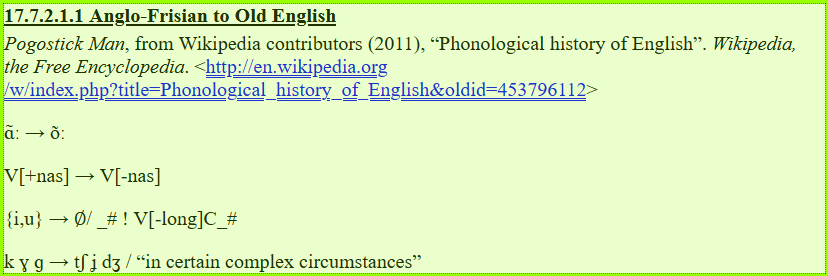
\includegraphics[width=\textwidth]{sidex.png}
  \end{frame}
  \begin{frame}{What were my goals?}
    \begin{itemize}
      \item What are the most common sound changes?
      \item How are sound changes influenced by their environments?
      \begin{itemize}
        \item More specifically: how do neighboring consonants affect vowel changes?
      \end{itemize}
    \end{itemize}
  \end{frame}
  \section*{Parsing the data}
  \begin{frame}{Parsing the data}
    \begin{columns}[c]
      \begin{column}{0.7\textwidth}
        \begin{itemize}
          \item The majority of my work
          \item Used a separate parsing script
          \item Lots of trial and error, running the parsing script over and over and fixing issues until nothing broke
          \item Had to manually edit the data a bit to remove things that would have made it impossible to parse
          \item Lots of complexity -- my explanation of the steps will be leaving out some of the edge cases I had to handle
        \end{itemize}
      \end{column}
      \begin{column}{0.3\textwidth}
        \centering
        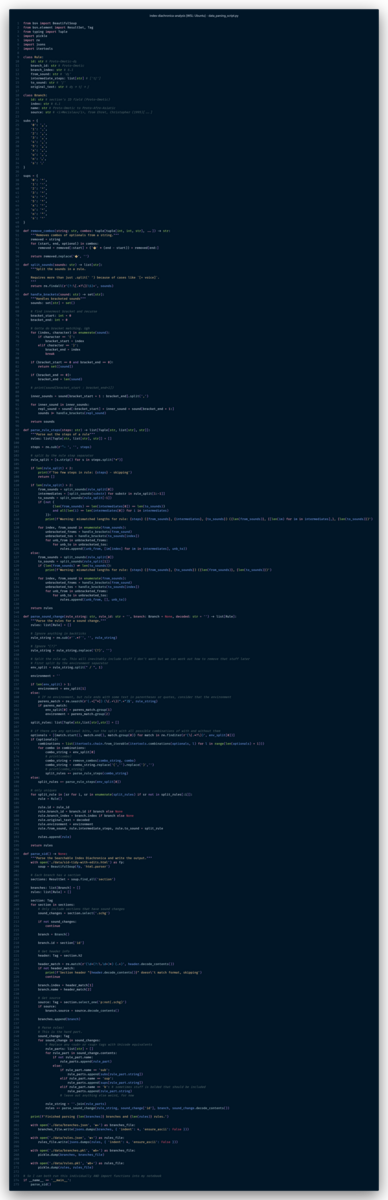
\includegraphics[width=0.8\textwidth, height=\textheight, keepaspectratio]{code1200.png}
      \end{column}
    \end{columns}
  \end{frame}
  \begin{frame}{Pulling the content from HTML}
    \begin{columns}[c]
      \begin{column}{0.5\textwidth}
        The first step was to pull sound changes from the HTML and clean up any extra HTML tags. This was done using \textbf{Beautiful Soup}. The data I wanted was the name of the branch, the branches' and sounds' IDs, and the full text of the sound change rule.
      \end{column}
      \begin{column}{0.5\textwidth}
        \centering
        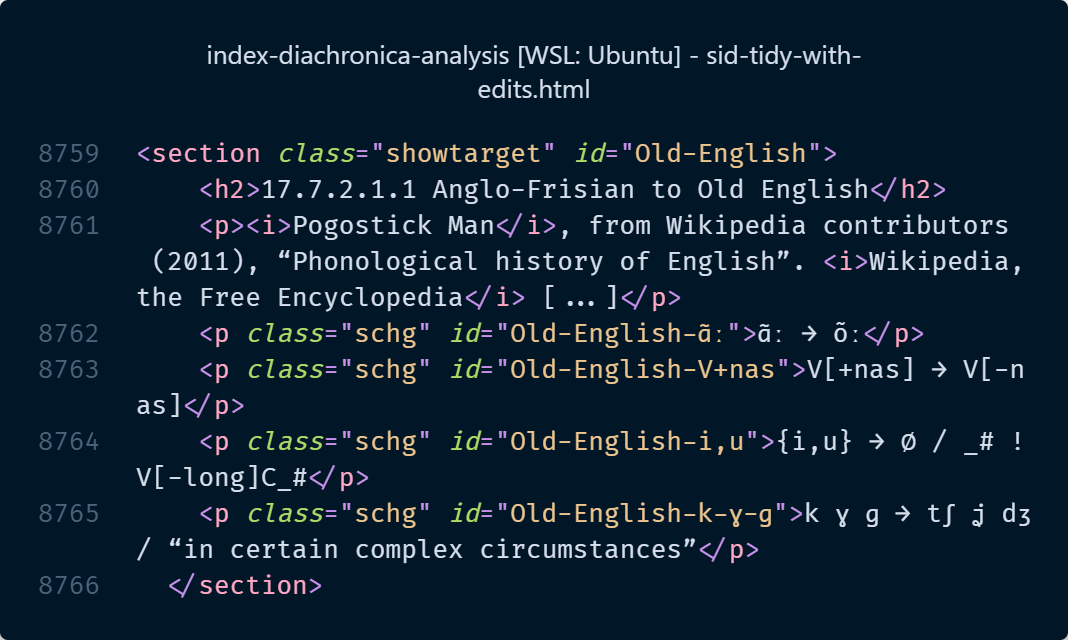
\includegraphics[width=0.8\textwidth, height=0.9\textheight, keepaspectratio]{html.png}
      \end{column}
    \end{columns}
  \end{frame}
  \begin{frame}[fragile=singleslide]{Pulling out the environment}
    \centering
    \verb|{i,u} → ∅ / _# ! V[-long]C_#|
    
    \vspace*{5pt}

    $\big\downarrow$

    \vspace*{5pt}

    \verb|_# ! V[-long]C_#|

    \vspace*{5pt}

    \begin{figure}
      \centering
      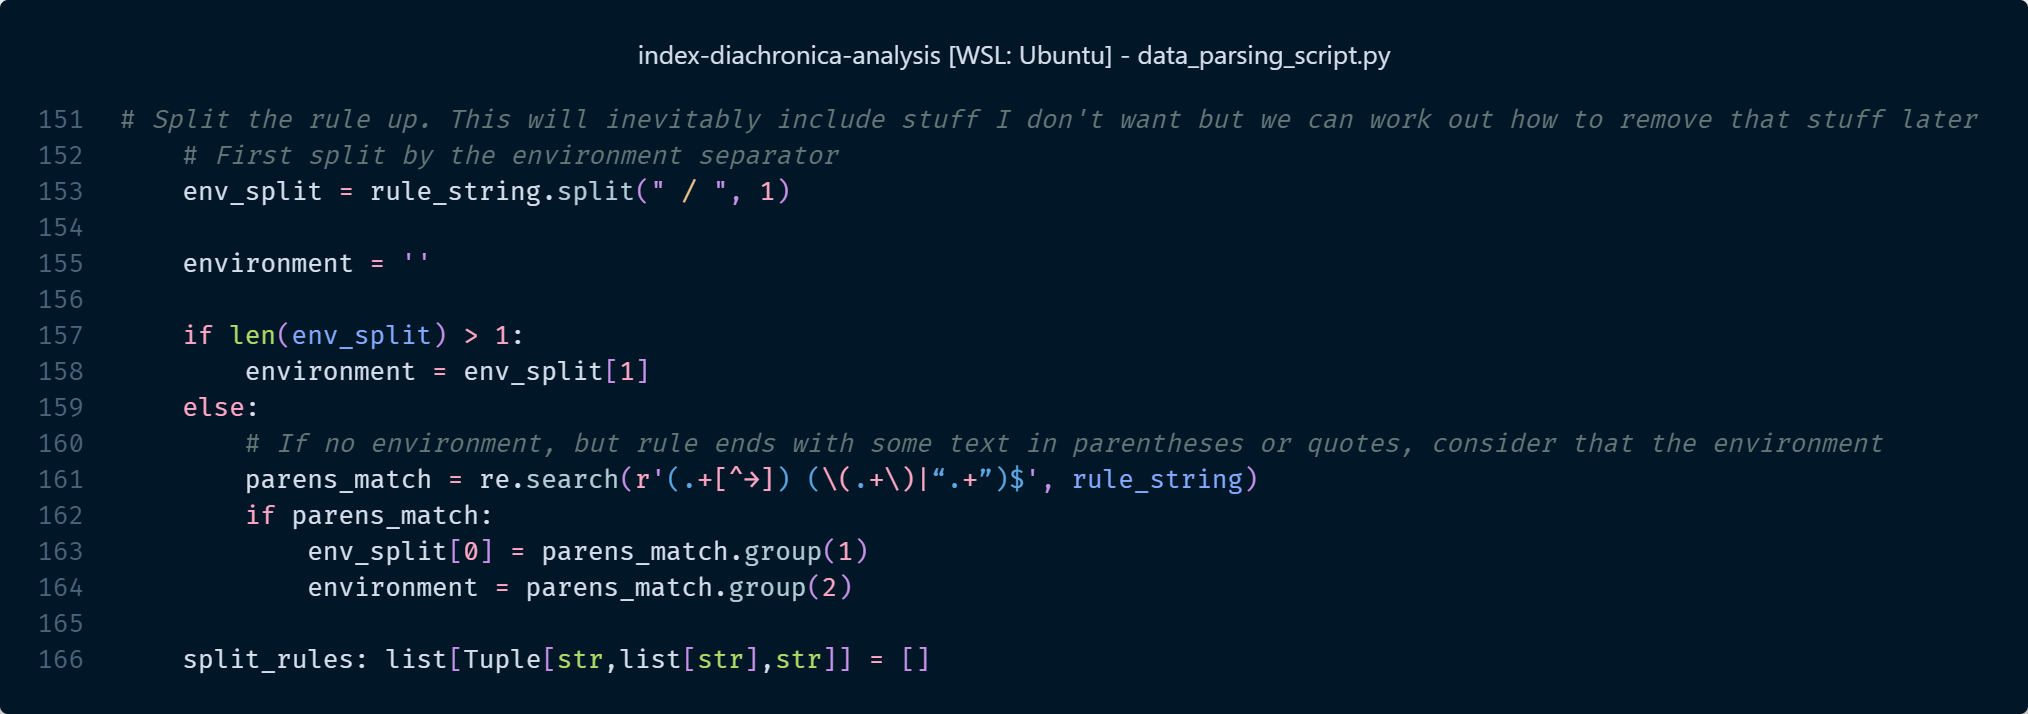
\includegraphics[width=1\textwidth, height=0.5\textheight, keepaspectratio]{env.png}
    \end{figure}
  \end{frame}
  \begin{frame}[fragile=singleslide]{Parsing ``optionals''}
    \centering
    \verb|e(ː)j → i|
    
    \vspace*{5pt}

    $\big\downarrow$

    \vspace*{5pt}

    \verb|ej → i|

    \verb|eːj → i|

    \vspace*{5pt}

    \begin{figure}
      \centering
      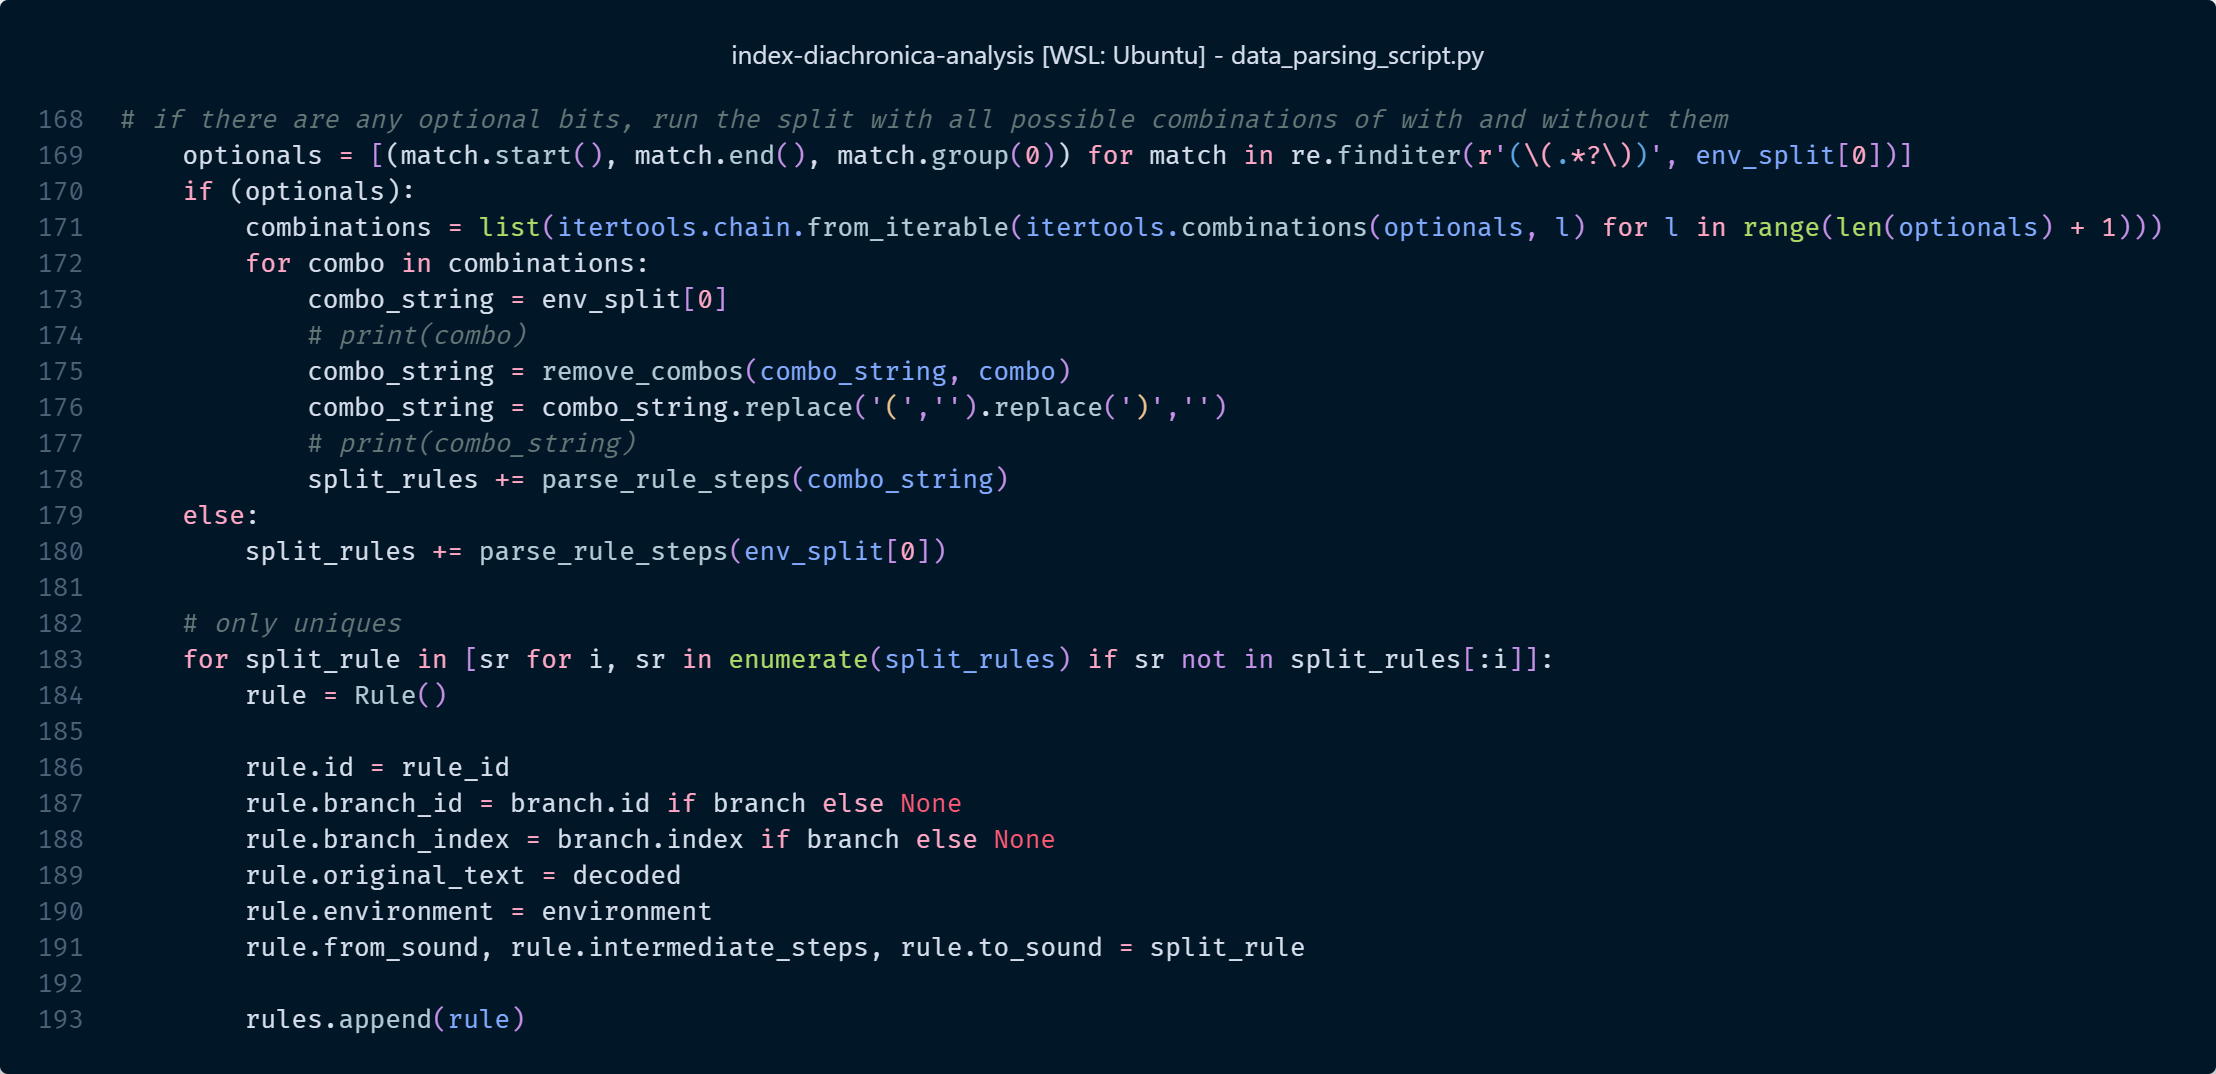
\includegraphics[width=1\textwidth, height=0.5\textheight, keepaspectratio]{optionals.png}
    \end{figure}
  \end{frame}
  \begin{frame}[fragile=singleslide]{Parsing steps and multi-sound rules}
    \centering
    \verb|aː ɔː → ɛː oː → eː ow → ej əw|
    
    \vspace*{5pt}

    $\big\downarrow$

    \vspace*{5pt}

    \scriptsize \verb|from_sound = "aː", intermediate_steps=["ɛː", "eː"], to_sound = "ej"|
    
    \scriptsize \verb|from_sound = "ɔː", intermediate_steps=["oː", "ow"], to_sound = "əw"|

    \vspace*{5pt}

    \begin{figure}
      \centering
      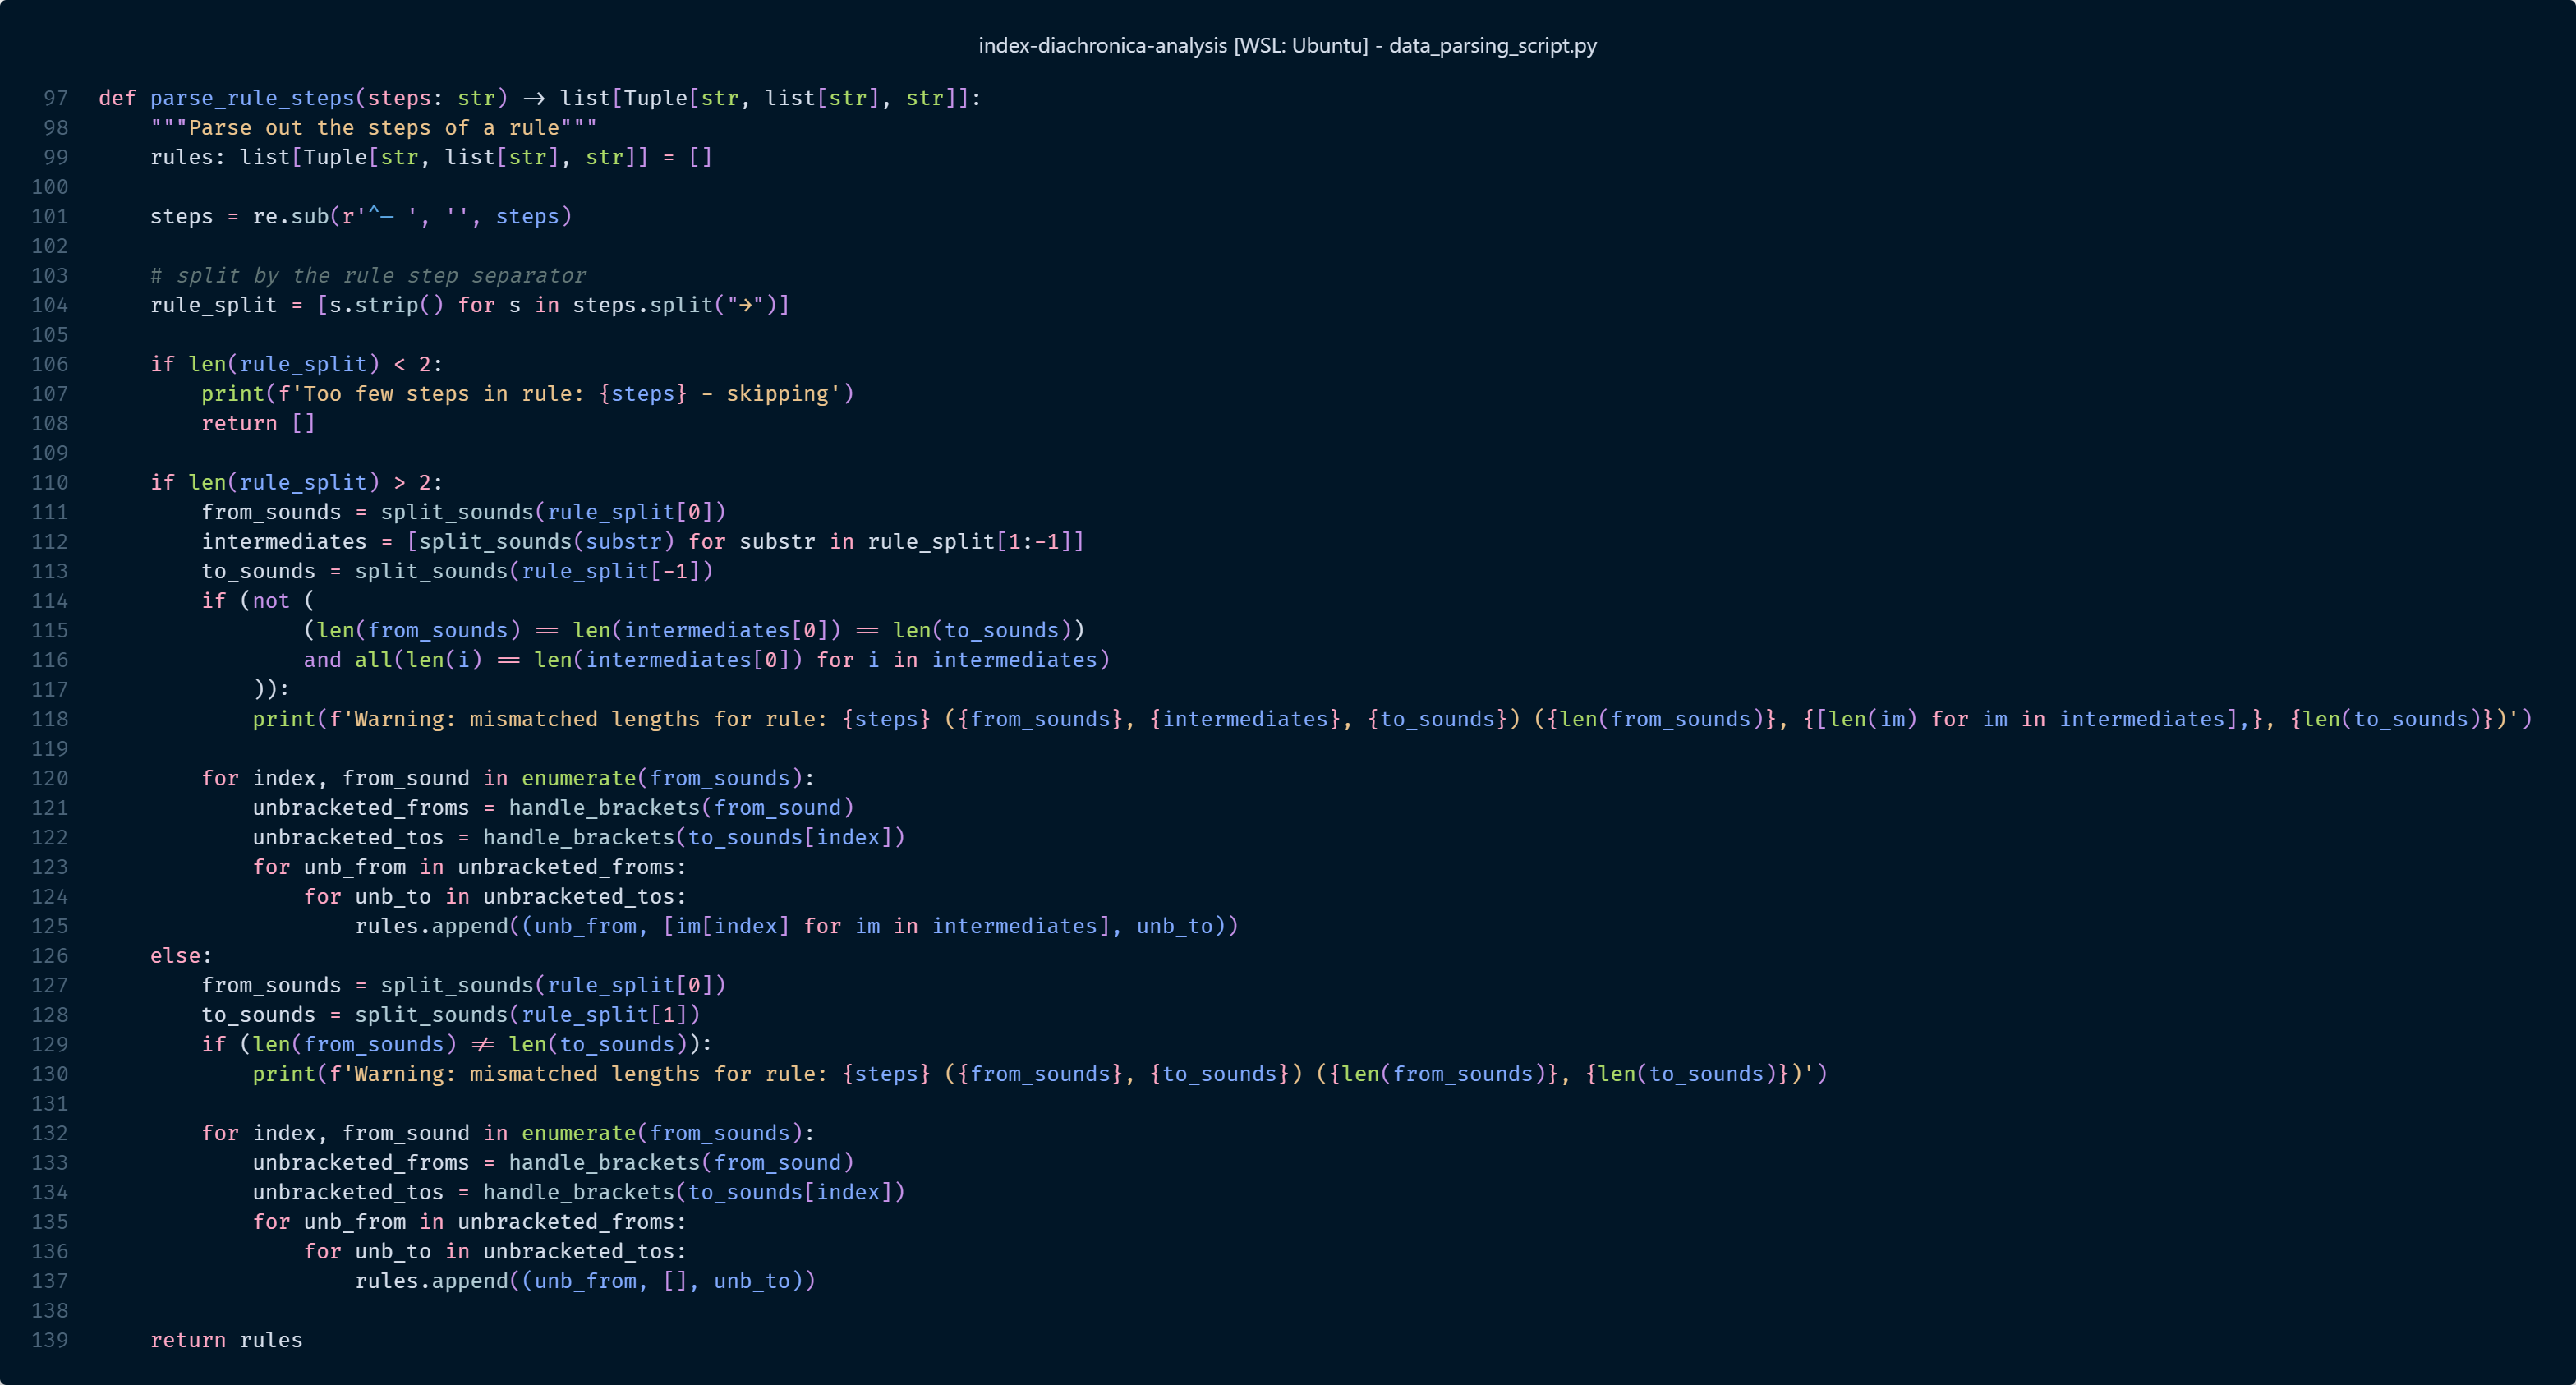
\includegraphics[width=1\textwidth, height=0.5\textheight, keepaspectratio]{steps.png}
    \end{figure}
  \end{frame}
  \begin{frame}[fragile=singleslide]{Parsing brackets}
    \centering
    \verb|{i,u} → ∅|
    
    \vspace*{5pt}

    $\big\downarrow$

    \vspace*{5pt}

    \verb|from_sound = "i", to_sound = "∅"|
    
    \verb|from_sound = "u", to_sound = "∅"|

    \vspace*{5pt}

    \begin{figure}
      \centering
      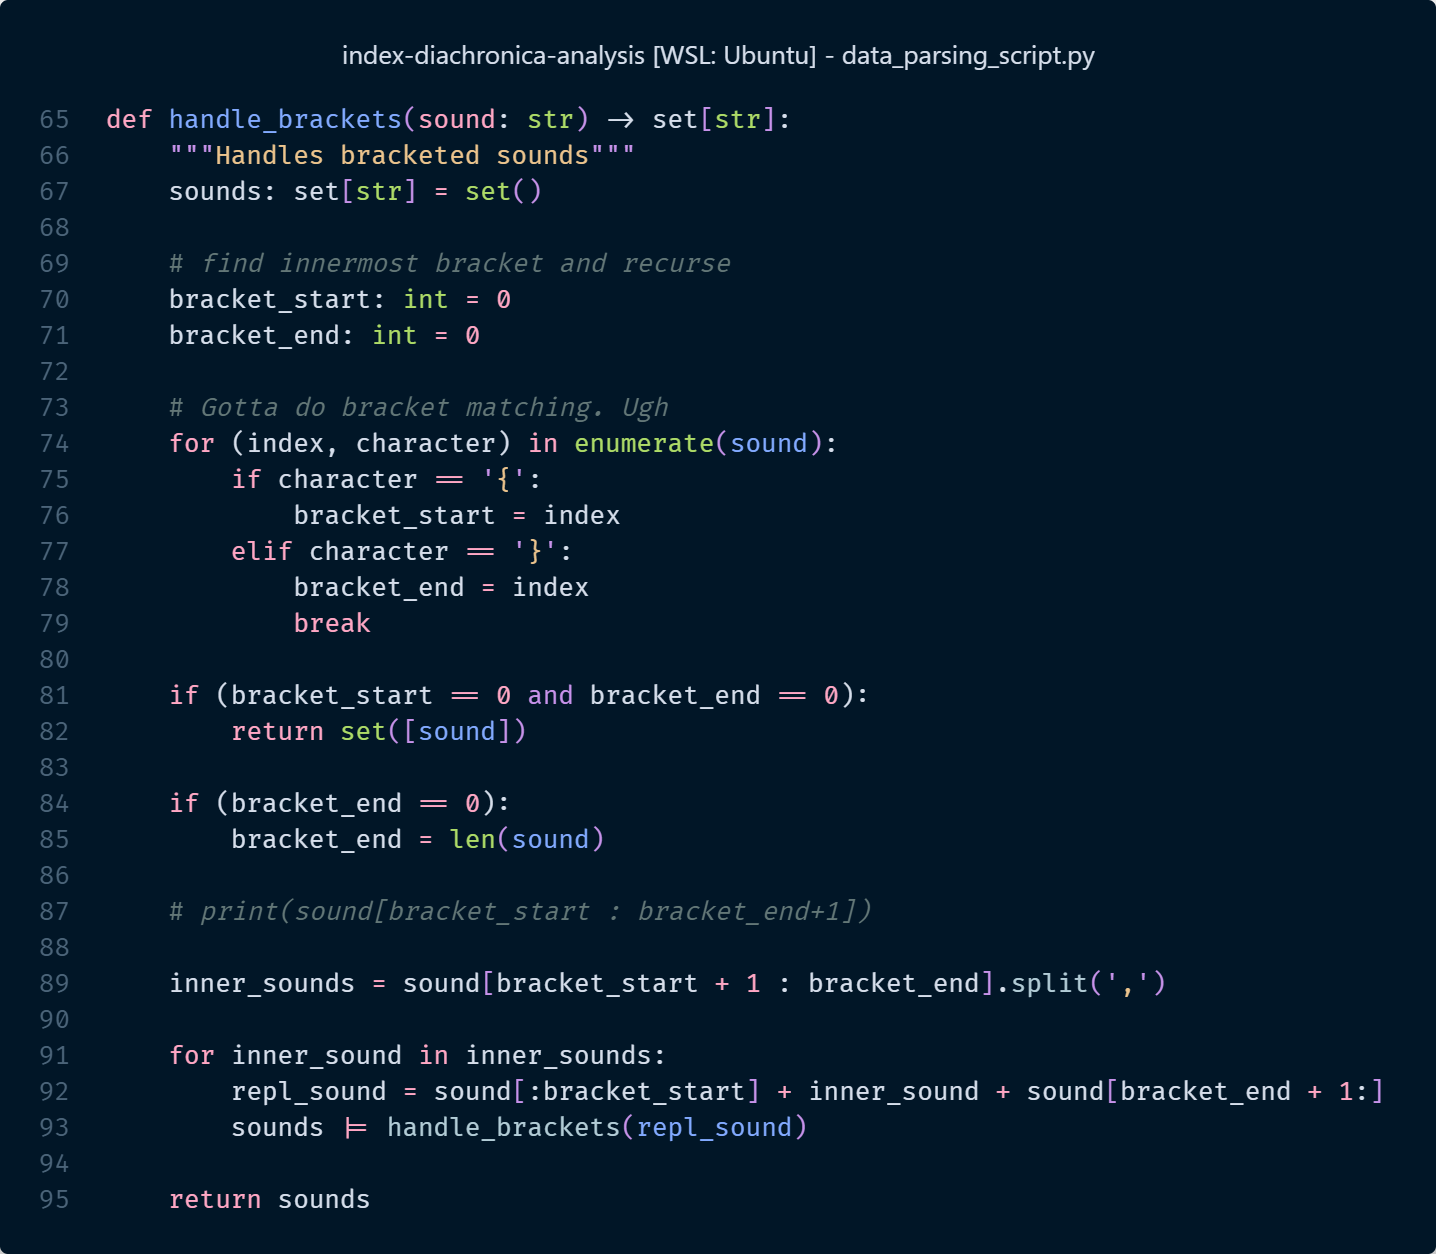
\includegraphics[width=1\textwidth, height=0.5\textheight, keepaspectratio]{brackets.png}
    \end{figure}
  \end{frame}
  \section*{What are the most common sound changes?}
  \begin{frame}{Questions to ask first}
    \begin{itemize}
      \item What does it mean for two sound changes to be `the same'?
      \begin{itemize}
        \item What if they have the same `from' and `to' sound, but different environments or intermediate steps?
        \item I looked at both options - considering these the same, and considering these different.
        \item Not much new information was gained by including environments or intermediate steps -- the results were just the `most common sound changes with no environment or intermediate steps'
      \end{itemize}
      \item Lots of sound changes are copied between different daughter languages in a single branch. Let's count those as just 1 sound change.
    \end{itemize}
  \end{frame}
  \begin{frame}[fragile=singleslide]{The most common sound changes}
    Looking at only the \verb|from_sound| and \verb|to_sound|... 
    \begin{columns}[c]
      \begin{column}{0.5\textwidth}
        \begin{table}
          \begin{center}
            \begin{tabular}{|c|c|c|}
              \hline
              \small \verb|from_sound| & \small \verb|to_sound| & \small \textbf{count} \\
              \hline
              h & ∅ & 46 \\
              w & ∅ & 44 \\
              ʔ & ∅ & 40 \\
              k & ∅ & 37 \\
              j & ∅ & 34 \\
              e & i & 34 \\
              a & e & 32 \\
              i & e & 30 \\
              u & o & 29 \\
              o & u & 29 \\
              \hline
            \end{tabular}
          \end{center}
        \end{table}
      \end{column}
      \begin{column}{0.5\textwidth}
        \begin{itemize}
          \item So many deletions! Makes sense, since what can be deleted is less limited than `what can become /i/'
          \item /h/ being removed is most common, which makes some sense -- i.e. British English ``history''
          \item Nothing really surprising here
        \end{itemize}
      \end{column}
    \end{columns}
  \end{frame}
  \begin{frame}[fragile=singleslide]{The most common sound changes}
    What if we ignore deleted sounds? 
    \begin{columns}[c]
      \begin{column}{0.5\textwidth}
        \begin{table}
          \begin{center}
            \begin{tabular}{|c|c|c|}
              \hline
              \small \verb|from_sound| & \small \verb|to_sound| & \small \textbf{count} \\
              \hline
              e &  i &  34 \\
              a &  e &  32 \\
              i &  e &  30 \\
              u &  o &  29 \\
              o &  u &  29 \\
              ts & s &  27 \\
              s &  ʃ &  26 \\
              ɡ &  k &  24 \\
              k &  ɡ &  23 \\
              a &  o &  23 \\
              \hline
            \end{tabular}
          \end{center}
        \end{table}
      \end{column}
      \begin{column}{0.5\textwidth}
        \begin{itemize}
          \item Still nothing too surprising here
          \item Mostly just simple vowel changes
          \item /ts/ → /s/ is the most interesting thing here
        \end{itemize}
      \end{column}
    \end{columns}
  \end{frame}
  \section*{How neighboring consonants affect vowel changes}
  \begin{frame}[fragile=singleslide]{More data parsing!}
    \begin{itemize}
      \item Filter down my rules to just vowel changes
      \item Pull neighboring consonants from the environment and/or rule
      \begin{itemize}
        \item Parse environments -- consonants before/after the underscore
        \item e.g. \verb|n_mV#| → \texttt{before = "n", after = "m"}
      \end{itemize}
      \item Used \textbf{Gruut IPA} to split strings of IPA characters into individual phones (\verb|/tʃuːz/| → \verb|/tʃ/ + /uː/ + /z/|)
      \item Used \textbf{ipapy} to break down phones into their component features:
      \begin{itemize}
        \item Consonants: voicing, place, manner, modifiers (palatalized, etc.)
        \item Vowels: length, height, backness, roundness, modifiers (centralized, etc.)
      \end{itemize}
    \end{itemize}
  \end{frame}
  \begin{frame}{How I performed the analysis}
    \begin{itemize}
      \item Assigned a number to the values of each vowel feature (0 = open, 3 = mid, 6 = close) and found the difference between start and end sound to get that feature's ``change''
      \item Looked at preceding and following consonants separately
      \item Did statistical t-tests to determine if the `average changes' for different consonant features were significantly different from each other, and in what direction they differed
      \item Visualized these results as a heatmap
      \item Outlined squares signify statistical significance
      \item Excluded duplicate sound changes shared by daughter languages within the same branch, like before
    \end{itemize}
  \end{frame}
  \begin{frame}{Place of articulation}
    \begin{figure}
      \centering
      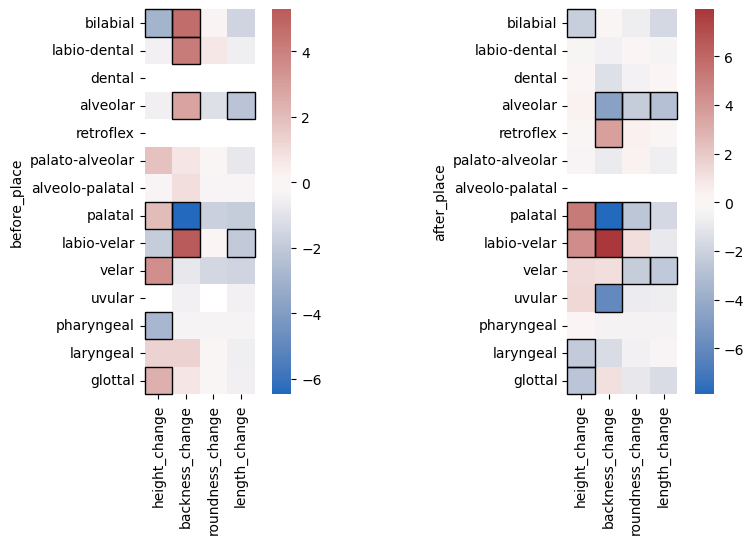
\includegraphics[width=\textwidth, height=0.7\textheight, keepaspectratio]{place_change.png}
      
      \scriptsize Height: negative = lowering (/u/ → /o/), positive = raising (/o/ → /u/)
      
      \scriptsize Backness: negative = fronting (/u/ → /i/), positive = backing (/i/ → /u/)
      
      \scriptsize Roundness: negative = unrounding, positive = rounding
      
      \scriptsize Length: negative = shortening, positive = lengthening
    \end{figure}
  \end{frame}
  \begin{frame}{Voicing}
    \begin{figure}
      \centering
      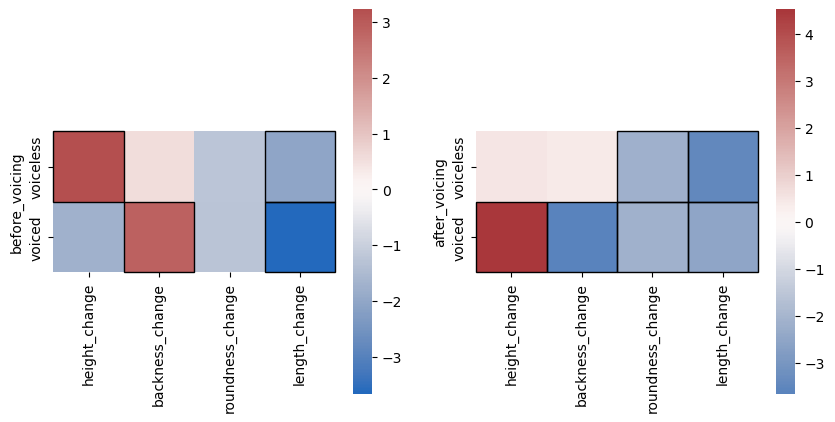
\includegraphics[width=\textwidth, height=0.7\textheight, keepaspectratio]{voicing_change.png}
      
      \scriptsize Height: negative = lowering (/u/ → /o/), positive = raising (/o/ → /u/)
      
      \scriptsize Backness: negative = fronting (/u/ → /i/), positive = backing (/i/ → /u/)
      
      \scriptsize Roundness: negative = unrounding, positive = rounding
      
      \scriptsize Length: negative = shortening, positive = lengthening
    \end{figure}
  \end{frame}
  \begin{frame}{Manner}
    \begin{figure}
      \centering
      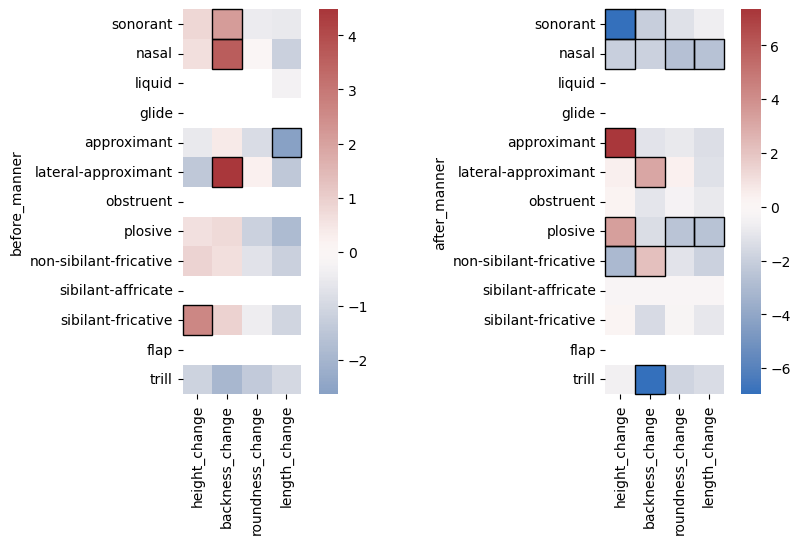
\includegraphics[width=\textwidth, height=0.7\textheight, keepaspectratio]{manner_change.png}
      
      \scriptsize Height: negative = lowering (/u/ → /o/), positive = raising (/o/ → /u/)
      
      \scriptsize Backness: negative = fronting (/u/ → /i/), positive = backing (/i/ → /u/)
      
      \scriptsize Roundness: negative = unrounding, positive = rounding
      
      \scriptsize Length: negative = shortening, positive = lengthening
    \end{figure}
  \end{frame}
  \begin{frame}{Takeaways}
    \begin{itemize}
      \item Some results lined up with what I expected (palatals are associated with fronting, /w/ is associated with backing) but I couldn't explain most results
      \item Each combination of features was not evenly distributed, so they might be contaminating each other's results
      \item I tried using linear regression to try and untangle this, but those results were even messier - not included here
    \end{itemize}
  \end{frame}
  \section*{Conclusion}
  \begin{frame}{Future ideas}
    \begin{itemize}
      \item Untangle the effects of these different variables to try and determine which features are actually having which effects
      \item Do the same analysis, but for consonant changes
      \item Fix some of the errors in my data -- there is a big PDF of corrections to the \textit{Index Diachronica} that someone has compiled
      \item Re-write the \textit{Index} using more standard notation, like PhoMo (a sound-change notation intended to be parsed by software and used to automatically apply sound changes to words)
      \item Interactive tools -- e.g. put in a word or IPA string, get the most likely ways that word could evolve
    \end{itemize}
  \end{frame}
  \begin{frame}[plain,c,noframenumbering]{Questions?}
    \centering
    \Large \textbf{Questions?}
  \end{frame}
\end{document}